\chapter{Anwendungsfall und Prototyp}
\label{chapter:prototype}

In den Kapiteln zuvor wurde in das Thema durch Grundlagen und eine Vorstellung der einzelnen Streaming frameworks eingeführt. Das Kapitel \ref{chapter:prototype} beschreibt eine Methode zur Messung der Performance. Es wird zunächst das Messverfahren gezeigt und die Messumgebung beschrieben. Abschließend wird eine Messung durchgeführt und die Messergebnisse vorgestellt.

In der Abbildung \ref{fig:prototypeStreamingGraph} wird ein erster Bildschirmausschnitt aus einer Messung mit Apache Storm über ein Standardtestdatensatz für das Zählen von Worten gezeigt.

\begin{figure}[htb!]
\centering
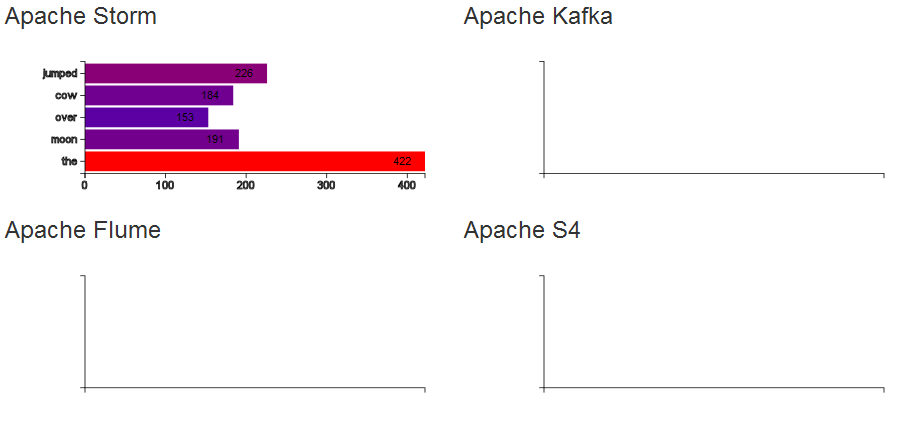
\includegraphics[width=1.0\textwidth]{bilder/PrototypeStreamingGraph.png}
\caption{Prototype Streaming Graph
\label{fig:prototypeStreamingGraph}}
\end{figure}

%STORM TRHOUGHPUT%
\begin{figure}
\begin{tikzpicture} 
\begin{axis}[ enlarge x limits=0.03, 
							%title=Messung,
							xlabel=$t$ in Sekunden,
							ylabel=Anzahl Nachrichten,
							axis x line=bottom,
							axis y line=left,
							ymin=0,
							ymax=2000000,
							width=1\linewidth,
							height=10cm,
							legend entries = {Storm HiPcRaw, Storm HiPcWordCount, Storm LoPcRaw, Storm LoPcWordCount},
							legend style={at={(1,1)},xshift=0.2cm,anchor=north east,nodes=right}] 
%nur punkte
%\addplot+[only marks, color=blue, mark options={scale=0.08}, mark=*] table [x=Time, y=Mps, col sep=comma,trim cells=true] {anhangMessung/traversedMeasure.log};
%verbundene Punkte
\addplot+[mark options={scale=0.07}, color=blue] table [x=Time, y=Mps, col sep=comma,trim cells=true] {anhangMessung/measureStormHighPcRaw.dat};
\addplot+[mark options={scale=0.07}, color=red] table [x=Time, y=Mps, col sep=comma,trim cells=true] {anhangMessung/measureStormHighPcWordCount.dat};
\addplot+[mark options={scale=0.07}, color=orange] table [x=Time, y=Mps, col sep=comma,trim cells=true] {anhangMessung/measureStormLowPcRaw.dat};
\addplot+[mark options={scale=0.07}, color=green] table [x=Time, y=Mps, col sep=comma,trim cells=true] {anhangMessung/measureStormLowPcWordCount.dat};
\end{axis} 
\end{tikzpicture}
\caption{Messung Apache Storm Nachrichtendurchsatz
\label{fig:messungStormNd}}
\end{figure}

%STORM CPU%
\begin{figure}
\begin{tikzpicture} 
\begin{axis}[ enlarge x limits=0.03, 
							%title=Messung,
							xlabel=$t$ in Sekunden,
							ylabel=CPU Auslastung in Prozent,
							axis x line=bottom,
							axis y line=left,
							ymin=0,
							ymax=1.5,
							width=1\linewidth,
							height=10cm,
							legend entries = {Storm HiPcRaw, Storm HiPcWordCount, Storm LoPcRaw, Storm LoPcWordCount},
							legend style={at={(1,1)},xshift=0.2cm,anchor=north east,nodes=right},
							yticklabel={\pgfmathparse{\tick*100}\pgfmathprintnumber{\pgfmathresult}\%},] 
%nur punkte
%\addplot+[only marks, color=blue, mark options={scale=0.08}, mark=*] table [x=Time, y=Mps, col sep=comma,trim cells=true] {anhangMessung/traversedMeasure.log};
%verbundene Punkte
\addplot+[mark options={scale=0.07}, color=blue] table [x=Time, y=SystemCpu, col sep=comma,trim cells=true] {anhangMessung/measureStormHighPcRaw.dat};
\addplot+[mark options={scale=0.07}, color=red] table [x=Time, y=SystemCpu, col sep=comma,trim cells=true] {anhangMessung/measureStormHighPcWordCount.dat};
\addplot+[mark options={scale=0.07}, color=orange] table [x=Time, y=SystemCpu, col sep=comma,trim cells=true] {anhangMessung/measureStormLowPcRaw.dat};
\addplot+[mark options={scale=0.07}, color=green] table [x=Time, y=SystemCpu, col sep=comma,trim cells=true] {anhangMessung/measureStormLowPcWordCount.dat};
\end{axis} 
\end{tikzpicture}
\caption{Messung Apache Storm CPU Auslastung
\label{fig:messungStormCpu}}
\end{figure}



%KAFKA TRHOUGHPUT%
\begin{figure}
\begin{tikzpicture} 
\begin{axis}[ enlarge x limits=0.03, 
							%title=Messung,
							xlabel=$t$ in Sekunden,
							ylabel=Anzahl Nachrichten,
							axis x line=bottom,
							axis y line=left,
							ymin=0,
							ymax=200000,
							width=1\linewidth,
							height=10cm,
							legend entries = {Kafka HiPcRaw, Kafka HiPcWordCount, Kafka LoPcRaw, Kafka LoPcWordCount},
							legend style={at={(1,1)},xshift=0.2cm,anchor=north east,nodes=right}] 
%nur punkte
%\addplot+[only marks, color=blue, mark options={scale=0.08}, mark=*] table [x=Time, y=Mps, col sep=comma,trim cells=true] {anhangMessung/traversedMeasure.log};
%verbundene Punkte
\addplot+[mark options={scale=0.07}, color=blue] table [x=Time, y=Mps, col sep=comma,trim cells=true] {anhangMessung/measureKafkaHighPcRaw.dat};
\addplot+[mark options={scale=0.07}, color=red] table [x=Time, y=Mps, col sep=comma,trim cells=true] {anhangMessung/measureKafkaHighPcWordCount.dat};
\addplot+[mark options={scale=0.07}, color=orange] table [x=Time, y=Mps, col sep=comma,trim cells=true] {anhangMessung/measureKafkaLowPcRaw.dat};
\addplot+[mark options={scale=0.07}, color=green] table [x=Time, y=Mps, col sep=comma,trim cells=true] {anhangMessung/measureKafkaLowPcWordCount.dat};
\end{axis} 
\end{tikzpicture}
\caption{Messung Apache Kafka Nachrichtendurchsatz
\label{fig:messungKafkaNd}}
\end{figure}

%KAFKA CPU%
\begin{figure}
\begin{tikzpicture} 
\begin{axis}[ enlarge x limits=0.03, 
							%title=Messung,
							xlabel=$t$ in Sekunden,
							ylabel=CPU Auslastung in Prozent,
							axis x line=bottom,
							axis y line=left,
							ymin=0,
							ymax=1.5,
							width=1\linewidth,
							height=10cm,
							legend entries = {Kafka HiPcRaw, Kafka HiPcWordCount, Kafka LoPcRaw, Kafka LoPcWordCount},
							legend style={at={(1,1)},xshift=0.2cm,anchor=north east,nodes=right},
							yticklabel={\pgfmathparse{\tick*100}\pgfmathprintnumber{\pgfmathresult}\%},] 
%nur punkte
%\addplot+[only marks, color=blue, mark options={scale=0.08}, mark=*] table [x=Time, y=Mps, col sep=comma,trim cells=true] {anhangMessung/traversedMeasure.log};
%verbundene Punkte
\addplot+[mark options={scale=0.07}, color=blue] table [x=Time, y=SystemCpu, col sep=comma,trim cells=true] {anhangMessung/measureKafkaHighPcRaw.dat};
\addplot+[mark options={scale=0.07}, color=red] table [x=Time, y=SystemCpu, col sep=comma,trim cells=true] {anhangMessung/measureKafkaHighPcWordCount.dat};
\addplot+[mark options={scale=0.07}, color=orange] table [x=Time, y=SystemCpu, col sep=comma,trim cells=true] {anhangMessung/measureKafkaLowPcRaw.dat};
\addplot+[mark options={scale=0.07}, color=green] table [x=Time, y=SystemCpu, col sep=comma,trim cells=true] {anhangMessung/measureKafkaLowPcWordCount.dat};
\end{axis} 
\end{tikzpicture}
\caption{Messung Apache Kafka CPU Auslastung
\label{fig:messungKafkaCpu}}
\end{figure}


Dataset: \citeint{dataset:shakespeare:1994:CWW}

%Virtualbox RAW MEssung%
\begin{figure}
\begin{tikzpicture} 
\begin{axis}[ enlarge x limits=0.03, 
							%title=Messung,
							xlabel=$t$ in Sekunden,
							ylabel=Anzahl Nachrichten,
							axis x line=bottom,
							axis y line=left,
							ymin=0,
							ymax=8000,
							width=1\linewidth,
							height=10cm,
							legend entries = {Raw VM1, Raw VM2},
							legend style={at={(1,1)},xshift=0.2cm,anchor=north east,nodes=right} ] 

\addplot+[mark options={scale=0.07}] table [x=Time, y=Mps, col sep=comma,trim cells=true] {anhangMessung/traversedMeasureRaw.dat};
\addplot+[mark options={scale=0.07}] table [x=Time, y=Mps, col sep=comma,trim cells=true] {anhangMessung/traversedMeasureRaw2.dat};
\end{axis} 
\end{tikzpicture}

\caption{Messung Nachrichtendurchsatz in Virtualbox
\label{fig:messungMaxNachrichten}}
\end{figure}



